\documentclass[12pt]{extarticle}
\usepackage[a4paper, margin=1in]{geometry}
\usepackage{graphicx} % Required for inserting images
\usepackage{dirtree}
\usepackage[edges]{forest}
\title{\textbf{SSL Project Report\\ WhatsApp Wrapped}}
\author{Parth Vartak \& Arnav Nigam}
\date{April 2026}
\bibliographystyle{unsrt}
\begin{document}

\maketitle
\tableofcontents
\pagebreak
\section{Introduction}
This is a project report about our work on the WhatsApp Wrapped SSL Project.
\section{External Libraries}
Certain external libraries were used in making of this project. They are listed here along with their purpose.
\begin{itemize}
    \item \texttt{numpy}: For array handling in chat generator and analyser.
    \item \texttt{random}: to generate random probability distributions required for chat generation.
    \item \texttt{datetime}: to work efficiently with dates and time while generating and analysing chat.
    \item \texttt{re}: to identify emojis using unicode.
    \item \texttt{json}: to use json file for data from chat to analyse it.
    \item \texttt{chart.js}: to make various charts and graphs to represent data in final wrapped website.
    \item \texttt{sys}: To include command line arguments in the python scripts
\end{itemize}
\section{Project Design}
\subsection{Directory structure}
Past versions of the directory are kept track of using git commits. An online GitHub repository is used for supporting independent development by collaborators as well. The GitHub repository is linked to the terminal using SSH key.\\ \\
\texttt{whatsapp-wrapped/}
\texttt{\begin{itemize}
    \item generator/chat.py
    \item parser/analyze.py
    \item web/
    \begin{enumerate}
        \item index.html
        \item styles.css
        \item app.js
        \item chart.js
    \end{enumerate}
    \item chat.txt
    \item data.json
    \item vocabulary.txt
\end{itemize}}
%\begin{figure}[h]
%    \centering
%    \includegraphics[width=0.7\textwidth]{directory.png}
%    \label{fig:placeholder}
%\end{figure}
\subsection{Design and Architecture}
Our project consists of a three-layer architecture which includes a Chat Generator (\texttt{chat.py}), a Chat Parser (\texttt{analyze.py}) and a Web Frontend made using HTML, CSS and JavaScript that together create a WhatsApp Wrapped Experience catered uniquely to the inputted chat.\\
The best part about the system architecture is that above three components are technically independent and can be used separately given the required inputs. \\
For example: if the analyzer is given a different chat in the required format as an input, then it also analyzes and stores the data that it will obtain after parsing that particular input file. Similarly, given an appropriate \texttt{JSON} file as an input to the \texttt{js} file, it would create a personalised WhatsApp Wrapped Experience for that particular chat.
The components:
\begin{enumerate}
    \item Chat Generator (\texttt{chat.py}): Takes a vocabulary file as an input (a csv file containing the desired vocabulary of words in it) and generates a chat (\texttt{chat.txt}) for the given time range and given personalities specified in the python script.
    \item Chat Parser (\texttt{analyze.py}): Takes in the \texttt{chat.txt} as input and then parses the file for the required statistics and outputs the data into a \texttt{JSON} file (\texttt{data.json}) which acts as the input for the next component.
    \item Web Frontend (\texttt{index.html}, \texttt{styles.css} and \texttt{app.js}): The HTML file specifies the structure of the website and its navigation patterns, whereas the CSS file adds all the beautifying design elements and transitions. The JS file makes the project dynamic, including details from the parsed chat in the form of \texttt{data.json} following a specific schema, and then renders charts, profile slides and other meticulously thought-over elements in the WhatsApp Wrapped 
    Experience.
\end{enumerate}
\begin{figure}
\centering
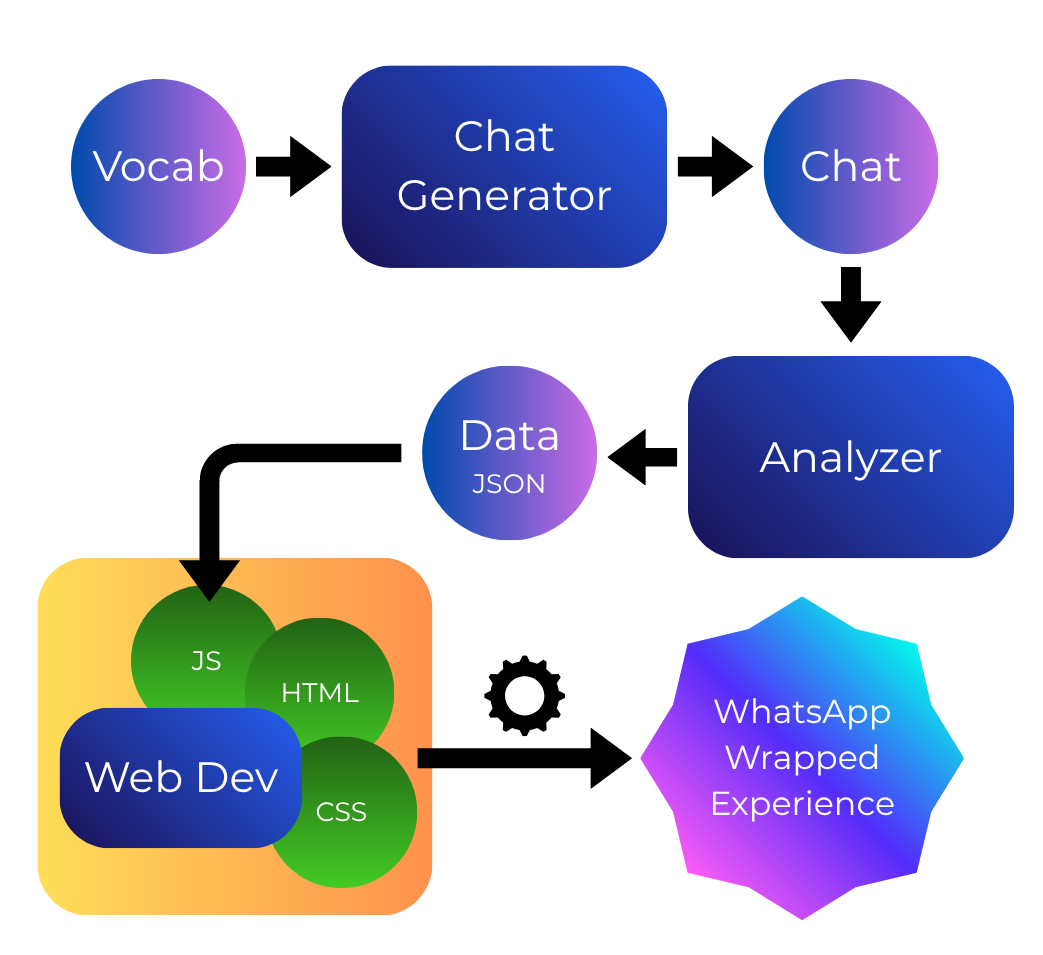
\includegraphics[width=0.75\textwidth]{flowchart.png}
\end{figure}
\subsection{Features Implemented}
\begin{enumerate}
    \item Chat Generator (\texttt{chat.py}): The Chat Generator involves creating 10 different personalities for the chat and then cutomising their messaging style working on their message length and their message times thus generating a model chat for roughly 100 days (starting from July 1, 2026) and the personalities we chose are as under:
    \begin{itemize}
        \item \textbf{Long Message User: } Uses relatively long messages most of the times, something around $40-50$ words being the probabilistically most common length (the length of message is chosen randomly from a biased array that weights higher towards longer messages)
        \item \textbf{Night Owl: } As the name suggests, this person is most active at night (defined in the code to be the time from 12 AM to 4 AM each day) and in general throughout the day has a slightly lower probability of messaging throughout the day at other times
        \item \textbf{Conversation Starter: } Most of the time initiates conversations, where initiating a conversation is defined as the time between two messages being greater than 0.8 times the upper bound of the time difference that we had chosen (these bounds on the time difference is different during night time and day time stated as 1s to 1200s during day time and 600s to 3600s during the night time, from which a value is randomly chosen to be the time duration before the next message)
        \item \textbf{Ghost: } This is the person who sends several messages consecutively as no one responds to the initial messages (ghosting) and thus the effect is seen as this person sending clusters of messages but the number of clusters is not too high and rather sparsely distributed so it is effectively like having several sufficiently time-separated clusters of messages throughout the chat
        \item \textbf{Emoji Talker: } This user uses emojis very frequently and otherwise has a normal messaging frequency just with each message having emojis as a significant fraction of it
        \item \textbf{Hype Person: } This person is the most active person in the group and sends the most number of messages and has the least average response time (roughly one-third of all others) and this has been implemented by multiplying the response time after each message to one-third of it when this person is chosen and also their probability of being chosen is much higher than the others
        \item \textbf{Long Vocabulary User: } Uses long words (defined as having length $\ge$ 12) very frequently in their messages
        \item \textbf{Editor: } Often (relative to others) edits their message which is characterised by the addition of ``[THIS MESSAGE WAS EDITED]" string after the message in the chat generator
        \item \textbf{Best Friends Pair: } A pair of Best Friends characterised by having the highest number of mutual direct replies. A direct reply is characterised by being the next adjacent message to the message being referred to
    \end{itemize}
    \item Chat Parser (\texttt{analyze.py}): The Chat Parser analyzes and stores all relevant parsed statistics by dumping them into the \texttt{data.json} file. The parser reads \texttt{chat.txt} line by line and extracts the relevant fields from each line and uses them to evaluate the statistics
    \item Web Frontend (\texttt{index.html}, \texttt{styles.css} and \texttt{app.js}): The \texttt{data.json} is read by the JavaScript file and elements structured out in the HTML and CSS files are dynamically modified.
    \begin{itemize}
        \item \texttt{index.html: } The HTML files contains a basic layout of the data-slides that are shown and just acts as a template to be filled by the JavaScript file. All elements are neatly designed using CSS from the \texttt{styles.css} file and serves as the structural framework for the actions to take place on
        \item \texttt{styles.css: } It contains all required styling and design elements that specify styles for the HTML framework. It contains styles for classes and ids mentioned in the HTML file.
        \item \texttt{app.js: } Adds all functionalities and dynamic updation of contents in the HTML file's structure such as:
        \begin{enumerate}
            \item Fetching and storing data from \texttt{data.json}
            \item Assigning Personality Tag
            \item Setting up floating words
            \item Setting up global statistics charts
            \item Profile Selection Page
            \item Fills in the values of the parsed statistics in the user profile page for each
            \item Heatmap showing time-of-the-day distribution
            \item Setting up the comparison table
            \item Functionalities of the Next and Back buttons
        \end{enumerate}
    \end{itemize}
\end{enumerate}
%also talk about custom stat here
%definition choices

\subsection{Code Structure}
\begin{enumerate}
    \item Chat Generator (\texttt{chat.py}) \cite{site1}: The code is overall divided into some sections (logical blocks) as follows:
    \begin{itemize}
        \item Making \texttt{vocab}: This part of the code is the beginning wherein the \texttt{vocabulary.txt} is read and tokenized, and then converted into a dictionary that stores the words with their corresponding token numbers. The use of token numbers makes it easy to choose words using \texttt{random} later in the code. Also in the very beginning the \texttt{chat.txt} file is set to empty so that on repeated runs of the chat generator, there is overwriting and not appending to previously stored text
        \item Personality specific functions: Starts off with initialising global variables and then moving on to define personality specific functions that skew probabilities when a particular person is chosen. The \texttt{pMod} function skews probability in favour of a person by a certain factor and is used to increase their probability of messaging after certain conditions are met. \texttt{LongVocab()}, \texttt{EmojiTalker()} and \texttt{LongMsg()} are functions that return the message string and they are the ones whose message content depends on the person. For others there is a general \texttt{printer()} function to print their messages which randomly chooses a length of the message from 1 to 17. The \texttt{NightOwl()},\texttt{ConvoStarter()}, \texttt{Ghost()}, \texttt{HypePer()} and \texttt{bestFrds()} functions just skew probabilities using the \texttt{pMod()} function for the required person after they meet certain conditions on time of the message or person who sent the previous message and so on. 
        \item \texttt{ChatGen()}: The main function that generates the Chat is \texttt{ChatGen()} which uses a \texttt{while} to iterate within a certain time range (the total time in seconds of the chat, which has been set as of now to 8400000 seconds). Within this, the functions that need to be always called are first called, such as \texttt{NightOwl()},\texttt{ConvoStart()},etc and then chooses a person from the given list of 10 people with probabilities being skewed as required. After this the person who has been chosen is then assigned a message and time of the message which is randomly chosen from \texttt{tmin} to \texttt{tmax} range. Then the line containing the person and time and the message in the required format is then written into the \texttt{chat.txt} file and also after that the edited message is selectively added to some messages
    \end{itemize}
    \item Chat Parser (\texttt{analyze.py}): The code is mainly divided into four file reading steps and parsing followed by dumping into \texttt{data.json}:
    \begin{itemize}
        \item First reading of \texttt{chat.txt}: Used to find the total number of lines and to set indices corresponding to each person in the chat, stored in a dictionary for access later, and also an inverse dictionary that gives us the person corresponding to an index
        \item Second reading of \texttt{chat.txt}: Splits the line into relevant blocks and parses the required block for all statistics (the main body of the parsing file)
        \item Third reading of \texttt{chat.txt}: Find the times of the first and last message and stores them as a \texttt{datetime} object for easy conditional calculations
        \item Fourth reading of \texttt{chat.txt}: This evaluates the time of the day distribution of messages for each person and thus generates a 3D array which is required for the Heatmap shown in each user's profile slides
        \item Assigning index to personality: After parsing the files for the required statistics we then assign each personality with the index of the person it corresponds to
        \item Dumping into \texttt{data.json}: The parsed information is dumped into \texttt{data.json}
    \end{itemize}
    \item \texttt{index.html}: It defines the structure for the slideshow. It contains the different slides categorised into sections numbered with \texttt{data-slide} numbers and are mostly empty except text that needs to be always shown. The empty regions or divs are then filled by \texttt{app.js}
    \item \texttt{styles.css}: For all elements defined in HTML and those that would be defined by JavaScript it contains their designing and styles
    \item \texttt{app.js} \cite{site2}: Majorly contains segments of the code containing global variable definitions, \texttt{init()} function which serves as the main function referring to most other function calls, functions to display parsed statistics' charts, displaying background floating words on start and end slides, setting up user profile selection, showing user profile, showing heatmaps and other charts for each user and comparison table. It also contains the event listeners added for Next and Back buttons as well as the functionalities of clicking on right one-third of the page to move ahead and left one-third to move back. Right and Left arrow keys can also be used.
\end{enumerate}

\section{Usage}
The chat generator, analyzer and final wrapped website are designed to work independently from each other. That is, the generator makes random chat and creates personalities for people independently of analyzer. The analyzer parses the chat text file and checks which user has which personality. The wrapped website represents this data and personalities in an visually appealing manner. The only connecting links are the \texttt{chat.txt} in 1st and 2nd, and \texttt{data.json} in 2nd and 3rd, which help in data transfer from one part of project to another. Analyzer is designed to work on any kind of chat, and the website will work for any data in the form of \texttt{data.json}.
For the Web Frontend, when it is fed with a suitable \texttt{data.json} file it works to produce a beautiful WhatsApp Wrapped Experience which has the following features and usage shown data-slide wise:
\begin{enumerate}
    \item The intro page, that has floating names in the background and the title in front with flashing text inviting to start the presentation. After this you click on the Next button
    \item The overall Global Statistics page which shows a basic overview of the number of messages as a doughnut chart, total number of people, total number of messages, total number of words used, busiest day and the longest silence. Proceed by clicking Next
    \item Line chart showing the Total number of words used by each person
    \item Bar chart of night messages per person
    \item Line chart of edited messages per person
    \item Pie chart of Conversations Started by each person
    \item Bar chart of emojis used per person
    \item Selection of profiles page, where you can choose to view a certain person or multiple people's profiles which is shown as green if selected
    \item After clicking next from the previous profile selection page, the main slideshow starts which shows each user's profile and their parsed statistics. Their bar chart of particular varieties of messages is shown and along with that there is a Heatmap which shows the activity of the user in the last 70 days
    \item After going through all selected profile slides one may choose to go back and select a different set, or move further to see the comparison table. The comparison table shows the major statistics of all selected personalities
    \item Then comes the final ending slide which contains in its background floating words (emotions) related to a friendly group chat
\end{enumerate}
\subsection{Execution}

\section{Retrospective}
\subsection{Challenges faced}
We faced many challenges and learned a lot while doing this project.
\begin{itemize}
    \item Choice of definitions of certain ambiguous terms such as direct replies
    \item Determining the probabilities to assign to each personality
    \item Figuring out how to manipulate the probabilities of each person when they are chosen
    \item Being rigorous enough at all places to be inclusive of edge cases and also ensuring that any file of the appropriate format can be used as an input
    \item Learning new functions for JavaScript implementation of some functions
    \item Ensuring a clean framework for the HTML file
\end{itemize}
\subsection{Given more Time}
\begin{itemize}
    \item Use a progress bar somewhere in the code for showing a statistic, as it looks quite good especially for statistics that need to show relative amounts
    \item Add more levels to the Heatmap colouring
    \item Implement NLP using NLTK to create meaningful sentences
    \item A select all button that automatically selects all people and similar functions that improve the user interface
\end{itemize}

\bibliography{references}
\end{document}
